%
% File acl2021.tex
%
%% Based on the style files for EMNLP 2020, which were
%% Based on the style files for ACL 2020, which were
%% Based on the style files for ACL 2018, NAACL 2018/19, which were
%% Based on the style files for ACL-2015, with some improvements
%%  taken from the NAACL-2016 style
%% Based on the style files for ACL-2014, which were, in turn,
%% based on ACL-2013, ACL-2012, ACL-2011, ACL-2010, ACL-IJCNLP-2009,
%% EACL-2009, IJCNLP-2008...
%% Based on the style files for EACL 2006 by 
%%e.agirre@ehu.es or Sergi.Balari@uab.es
%% and that of ACL 08 by Joakim Nivre and Noah Smith

\documentclass[11pt,a4paper]{article}
% \usepackage[utf8]{inputenc}
\usepackage[hyperref]{acl2021}
\usepackage{times}
\usepackage{float}
\usepackage{latexsym}
\usepackage{graphicx}
\renewcommand{\UrlFont}{\ttfamily\small}

% This is not strictly necessary, and may be commented out,
% but it will improve the layout of the manuscript,
% and will typically save some space.
\usepackage{microtype}

\aclfinalcopy 

%\setlength\titlebox{5cm}
% You can expand the titlebox if you need extra space
% to show all the authors. Please do not make the titlebox
% smaller than 5cm (the original size); we will check this
% in the camera-ready version and ask you to change it back.

\newcommand\BibTeX{B\textsc{ib}\TeX}

\title{Understanding Idiomatic Expressions}

\author{Vinay Kaundinya Ronur Prakash \\
  Mtr. Num 6905228 \\
  University of Paderborn, Paderborn, Germany \\
  \texttt{vinay@mail.uni-paderborn.de} \\}

\date{}

\begin{document}
\maketitle
\begin{abstract}
  This report addresses two of the most challenging tasks in NLP, partaining to langauge learning in specific and applications like sentiment analysis, machine translation etc in general.
  Case studies reveal that a good percentage of non native language speakers have limited knowledge of collocations. A 3 staged system was proposed that can automatically detect unexpected collocations in learner corpus. The implemented model is then evaluated at each stage to derive potential areas of improvement.
  We then introduce the second challenge of disambiguating potentially idiomatic expressions. Related past works reveal the usage of directional word embedding models in earlier works. However we discuss a BERT based methodology, that uses bidirectional contextual embeddings to disambiguate a PIE in a given context. 
  We use the BERT model in both supervised and unsupervised settings and results show that the proposed method outperforms previous state of the art. 
  To conclude, we discuss some sources of errors and pointers for future work.  
\end{abstract}

\section{Introduction}
One of the challenging areas with researchers concerned is second language(L2) or foreign language teaching and learning. It is estimated that about 750 million people in the world speak English as a second language, compared to 375 million native English speakers \cite{li-gaillat-2020-automatic}. 
The Center for Educational Statistics estimates that about 67$\%$ students in public schools as well as a large number of international students in colleges and universities around the world have limited English language proficiency, 
(Burghardt 2002 CITE HERE). These data emphasize the growing need for assistance for non-native language speakers.

Various studies have found that knowledge of phrases and more specifically Multiword Expressions is an important part of language learning and in being able to communicate like native language speakers. 
Zhang (1993 CITE HERE) conducted 2 writing tests to test the knowledge of multiword expressions on 30 native and 30 non-native speakers of English, all of whom were college freshmen. 
In both tests, native speakers significantly outperformed the non native speakers. Zhang concluded that knowledge on multiword expressions is a source of fluency in written communication among language learners. 

Different types of errors were made by non-native speakers, some of which are usage errors, such as prepositions or collocations. Collocations are defined as words co-occurring within a short space of each other (e.g. “doing the dishes”, “salt and pepper”) (Sinclair, 1991 CITE HERE).
Nguyen and Webb(CITE HERE) devised a test to examine the relationship between the knowledge of English lexical collocations and the general English proficiency of 368 student participants at a Vietnam Univeristy. 
187 were female and 181 were male participantsand all of them had learnt English as foreign language for more than 5 years at high school equivalent level. The results showed that more than 50$\%$ of students had failed to guess the correct answers indicating poor language proficiency.
While the density of collocation can vary within text or speech, an uncommon combination of words such as "powerful tea" instead of "strong tea" can disrupt communication. Therefore, it would be advantageous for L2 learners to have automatic detection and correction of erroneous collocations. 
One such system with right feedback messages can be used to guide students in their meta-cognitive learning process.

A multiword expression can be idiomatic in the sense that its meaning cannot be derived from the meanings of its components. The majority of multiword expressions can be interpreted as figuratively or literally in different contexts. 
A terminological problem is posed by idiomatic expressions like "wake up and smell the coffee", which is suitable when they are used in their idiomatic or figurative sense, but not so much when they are used in a literal sense. 
Determining the correct meaning of such multiword expressions in context is shown to be crucial for many NLP downstream tasks like sentiment analysis, automatic spelling correction and machine translation. A new term has been coined for such multiword expressions as "Potentially Idiomatic Expressions" or PIEs.

Through the course of this article we look at some solutions for the challenges mentioned above. We look at an approach proposed by (Jen-Yu Li et al CITE HERE) for automatic detection of unexpected/erroneous collocations in learner
corpus. We then discuss a solution proposed by authors (Murathan Kurfalı et al CITE HERE) for determining the correct meaning of potentially idiomatic expressions.

\section{Related Work}

We consider detection of erroneous collocations and disambiguating potentially idiomatic expressions based on the context it appears as two main problems. Under this section we look at some of the methods, approaches and models that have laid foundation for further works in the scope of the two problems. 

Authors of the paper (CITE C HERE) observe that second language learners usually have problems with collocations and correction of such erroneous collocations can help learners increase their competence their proficiency in English language writing. Hence they report some of the earlier works that were made in detection of erroneous collocations. 
According to some researchers (Nesselhauf, 2003; Hong et al., 2011), collocation errors are related to the learner's first language(L1). Past work reveals that, systems that have automatic detection and correction of erroneous collocations is based on both a learner corpus (used to extract known collocational errors), 
and a reference corpus (used to extract standard collocations). 

On similar lines, authors Chang et al.(CITE HERE) explored a method of extraction based on a bilingual collocation corpus, leveraging its capability to provide phrasal translation memory. In spite of the approach's exceptional performance (precision= 0.98, recall=0.91), 
the limitation of this approach lies in the requirement of a bilingual dictionary, a parallel corpus for a specific L1 and  L2 (English for example), as well as word-alignment matching of translations. These works in the past forms the foundation and makes way for better approaches in automatic detection of erroneous collocations.

The second problem that we delve deep in is the challenge of disambiguating potentially idiomatic expressions(PIEs). In achieving the same a number of approaches from employing linguistic features to more neural approaches, have been proposed in the recent times. One of the earlier works that came up with a generalized method instead of methods for individual idioms was proposed by Sporleder and Li (2009)(CITE HERE). 
In this work cohesion graphs was employed and the authors hypothesized that if exclusion of a PIE improved the cohesion in general then the excluded PIE was used figuratively. Authors trained a supervised classifier to classify data in a dataset consisting of high confidence instances. 

While authors Rajani et al. (2014) train a L2 regularized Logistic Regression (L2LR) classifier on a variety of features including bag of words, some works adopt an ensemble learning approach that considers three different classifiers trained on different representations of the context of a token. 

Among various works, research by Wiedemann et al. (2019) successfully used the contextual embeddings to solve the problem of word sense disambiguation(WSD) using BERT. Results of this work demonstrates that BERT embeddings can be used to form clusters for different senses of a given word in various contexts and thus BERT looks to be contextual as it claims to be. 

\section{Detection of Erroneous Collocations}

As we have seen earlier, it is clear to us that proficiency of multiword expressions is crucial in language learning for non native speakers. We have also seen that collocational errors is one of the common mistakes made by learners. Here we look at a state of the art approach proposed by (CITE C HERE), that provides us a methodology for helping language learners by automatic detection of unexpected or erroneous collocations.

\begin{figure}[H]
  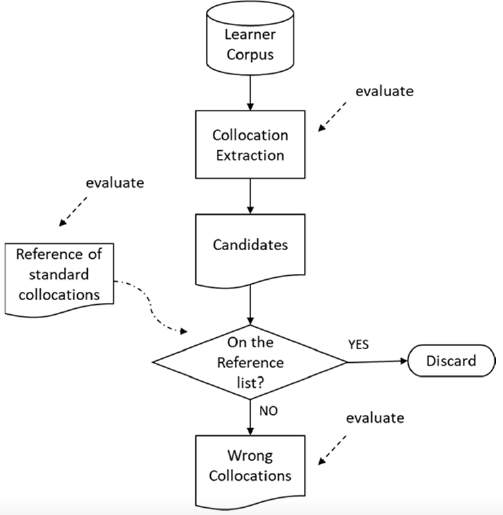
\includegraphics[width=8cm, height=9cm]{gfx/collocation_system}
  \caption{Proposed system design for erroneous collocation extraction in stages}
  \label{fig:colloc_sys}
\end{figure}

The proposed approach extracts erroneous or unexpected collocations in the following 3 stages:
\begin{itemize}
  \item Implementation and evaluation of a collocation extraction module
  \item Collection of standard collocations from a native corpus
  \item Extraction of wrong collocations from a learner corpus
\end{itemize}
The basic idea is to extract all possible collocations from a learner's corpus. These learner collocations are then compared to a standard collocations list from a native corpus(extracted previously). The collocations that do not match the collocations in the standard list are considered as wrong collocations. The system architecture in figure \ref{fig:colloc_sys} also shows the evaluation points of the model at the end of all the 3 stages. 

\subsection{Methodology}
In the following sections we take a look at a more detailed level of each the 3 stages of erroneous collocations extraction.

\subsubsection{Collocation Extraction Module}
The authors first implement the collocation extraction module. Authors use a PARSing and Multi-word Expressions (PARSEME2) corpus for extracting collocations using the implemented module, whose results was later on stored as PARSEME list. Based on reaserch by According to Garcia et al. (2019), authors also regard Light Verb Constructions (LVCs) in VN (verb + noun) form as collocations. 

These LVCs were manually annotated with the help of language experts. These LVCs were then capture as PARSEME LVC list. The PARSEME LVC list, now acts as the ground truth or gold standard for evaluating the first stage. 

\begin{figure}[H]
  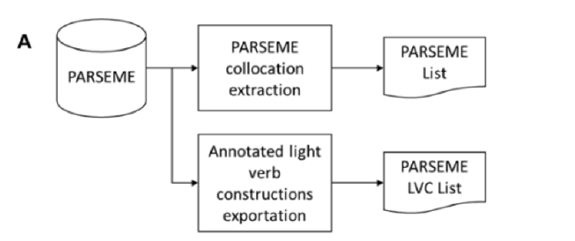
\includegraphics[width=8cm, height=4cm]{gfx/c_stage_1.png}
  \caption{PARSEME list is generated using implemented module and PARSEME LVC list is used for first stage evaluation.}
  \label{fig:c_stage_1}
\end{figure}

\subsubsection{Collection of Standard Collocations}
In this stage, authors prepare a list of standard collocations. In order to make an elaborate list of standard collocations, they used the module from stage 1 to extract collocations from British National Corpus (BNC). The extracted collocations forms the BNC list. This list merged with the previously obtained PARSEME LVC list. 

\begin{figure}[H]
  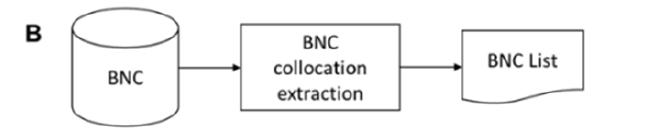
\includegraphics[width=8cm, height=2cm]{gfx/c_stage_2.png}
  \caption{BNC list is now combined with PARSEME LVC list to get a gold standard collocation list.}
  \label{fig:c_stage_2}
\end{figure}

Since any kind of errors in the gold standard list would result in decreased performance of the module, the gold standard list was annotated manually by language experts. 

\subsubsection{Extraction of Wrong Collocations}
Here the authors extract candidate collocations from the available National University of Singapore Corpus of Learner English (NUCLE4) to create a list named as the NUCLE List. Then the wrong collocations, along with collocations of VN form were detected in sentences. These sentences were manually annotated with erroneous collocations
(Wci tag) and were exported. The erroneous collocations were then saved as NUCLE WC List. It was used to evaluate the overall performance of our system.

\begin{figure}[H]
  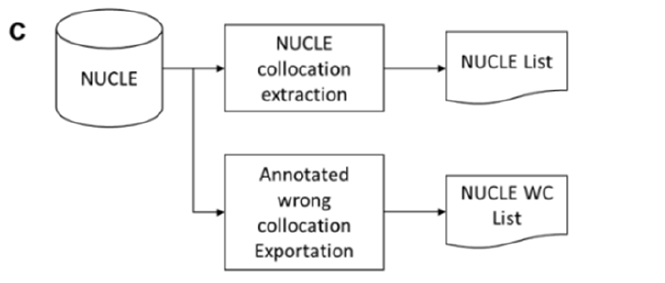
\includegraphics[width=8cm, height=4cm]{gfx/c_stage_3.png}
  \caption{Shows the extraction of candidate collocations from NUCLE.}
  \label{fig:c_stage_3}
\end{figure}

Python was used to write scripts with Natural Language Toolkit (NLTK). Five lexical association measures were used in collocation extraction tasks, namely the raw frequency
counting, t-test, chi-square test, log likelihood ratio, and pointwise mutual information.

\subsection{Results and Evaluation}
Under this subsection we look at how each of the 3 stages of the proposed methodology is evaluated. We also look at the $F_1$ and $F_{0.5}$ scores and compare the results of different lexical measures.

In the collocation extraction stage, PARSEME LVC list is used as the ground truth and is them compared to entries in PARSEME list. Using raw frequency measure, authors achieved the best precision rate of $0.11$ for bigram detection with a minimal frequency of $2$. In case of top 300 collocations, best $F_1$ and $F_2$ scores achieved are both $0.08$.

The BNC list that we extract in the second stage is evaluated manually with the help of an language expert. An English teacher was given a random sample of 200 samples from the BNC list to be annotated. He also consulted Corpus of Contemporary American English (COCA) collocate search tool, in case of not so obvious cases. The final precision is noted around $0.57$.

\begin{figure}[H]
  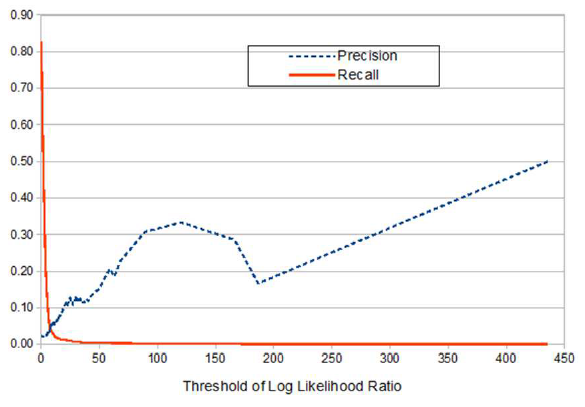
\includegraphics[width=7cm, height=5cm]{gfx/c_result_1.png}
  \caption{Shows the global view of precision and recall values versus different thresholds}
  \label{fig:c_result_1}
\end{figure}

As the last step deals with extraction of wrong collocations, we check the intersection between the standard collocations list(PARSEME LVC $\cup$ BNC) and the extracted wrong collocations(NUCLE WC) is a null set. It was noted that there about 11 collocations in common between NUCLE WC List and the PARSEME LVC, about 20 collocations in common between the NUCLE WC List and the BNC List and about 4 collocations as an intersection of all 3 lists. 
Thus a total of 27(20 + 11 - 4) common collocations that amounts to $1.8\%$ of NUCLE WC list.

\begin{figure}[H]
  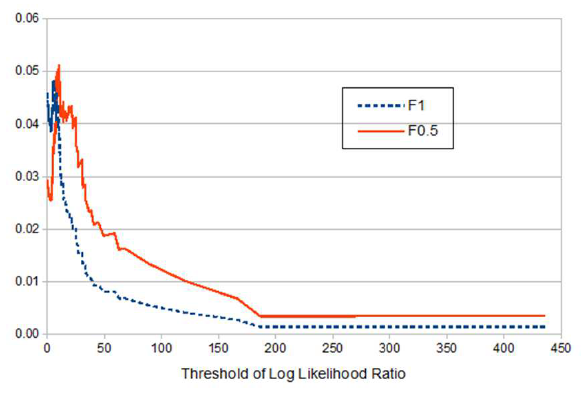
\includegraphics[width=7cm, height=5cm]{gfx/c_result_2.png}
  \caption{Shows the global view of $F_{1}$ and $F_{0.5}$ scores versus different thresholds}
  \label{fig:c_result_2}
\end{figure}

Authors also look to optimize by selecting a log likelihood ratio, the precision and recall were observed to be $0.04$ for a threshold set to 8 (only 1408 candidates were extracted). Figure \ref{fig:c_result_1} shows how recall and precision values vary for different thresholds. Maximum recall($0.83$) is achieved when all the candidates (54,471) are extracted, however it results in very low precision($0.02$). $F_{0.5}$ score reaches its peak of 0.05 for a threshold of 8 to 10, but $F_{1}$ score varies between 0.04 to 0.05 as demonstrated in Figure \ref{fig:c_result_2}. The optimal log likelihood ratio threshold is set to 8 in the experiments.

\section{Disambiguation of PIEs}
The other important challenge that we have recognized in language learning is to distinguish the difference between the literal sense and figurative sense of known potentially idiomatic expressions(PIEs). Input to such systems would be a set of sentences with target PIEs. Regarding the current problem as a word sense disambiguation problem, authors make a basic assumption that the context in which a PIE occurs literally and figuratively are distinct enough from each other to be assigned a fundamentally different contextual representations. In the following sections we look into a brief introduction of the contextual language model BERT that is used in all the experiments, classifiers used in case of supervised and unsupervised classification scenarios.

\subsection{BERT}
BERT is a multi-layer Transformer encoder based language model and stands for Bidirectional Encoder Representations for Transformers. Upon reading the input, a directional Transformer model processes the input only in one direction(either from left to right or vice versa). However a BERT model processes the input sentence from both the sides (left to right and right to left) in order to model the context of a word. BERT uses special tokens like $"[$CLS$]"$ (at the beginning of a sentence) and $"[$SEP$]"$ token (at the end of each sentence), thus indicating sentence boundaries as shown in Figure \ref{}.

\begin{figure}[H]
  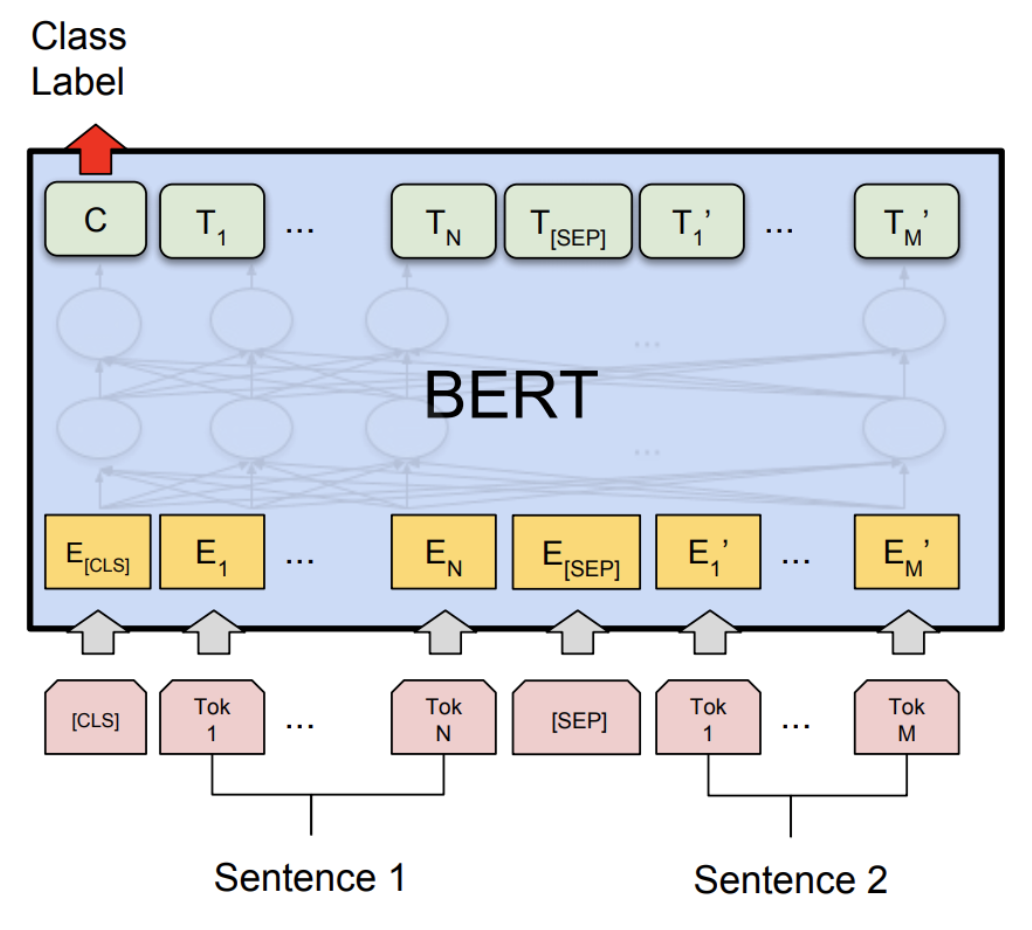
\includegraphics[width=7cm, height=5cm]{gfx/bert1.png}
  \caption{An instance of BERT that takes a pair of sentences as input}
  \label{fig:p_bert1}
\end{figure}

To overcome challenges in a typical directional model, BERT uses two training strategies:

\begin{itemize}
  \item Masked Language Modelling (MLM): In order to improve the context sensitivity of the model, new special token called $"[$MASK$]"$ is introduced. About $15\%$ of the input tokens are randomly
  replaced with a special “[MASK]” token. MLM forces BERT to consider the context of a word from both the sides of a sentence.

  \item Next Sentence Prediction (NSP): We know that the input to BERT is sentence pairs, and half of the time the second sentence is randomly selected from the given corpus. Primary objective of NSP is to determine whether the second sentence passed as input follows the first sentence in the original text and uses to binary classification to achieve the task. 
\end{itemize}

\subsection{Supervised setting}
In a typical case of supervised classification, the model is made up of an encoder followed by a classifier. Encoder is responsible for assigning a unique representation for each token reflecting their complete context. Authors use two types of encoders in their experiments, Monolingual BERTs and Multilingual BERT (mBERT).

Monolingual BERTs used here have the same architecture,  they are made up of 12 transformers layers and trained on huge monolingual corpus. Two monolingual BERTs used are bert-base-cased and German-Bert(trained on German language corpus).

104 Wikipedia dumps with shared word-piece vocabulary were concatenated to forma huge corpus and the same is used to train mBERT. 

In order to count for BERTs internal tokenizer that might split some words(eg. 'microscope') into multiple tokens('micro' + 'scope'), we first prepare a word-token map that can keep track of each PIE and the words it is split into. Each PIE is then represented by averaging their each word representation. Formula for the same is as follows,

\begin{equation}
  \label{equ:1}
  V_{PIE_{i}} = \frac{1}{k}\sum_{j=1}^{k} v_{i,j}
\end{equation}

k is the number of word pieces that PIE is split into, $v_{i,j}$ is the representation of the jth word piece in the ith sentence in the dataset.

Some PIEs like “broke a leg” can be more likely to be used with the literal sense as opposed to “break a leg” which is almost always used figuratively. This shows that some PIEs display larger variation of inflectional forms than their idiomatic variation. To control this variation, we lemmatize the words of PIEs before passing as encoder input. 
We do not do the same in case of German PIEs as one word or two words is a strong indicator of its sense. We finally use a simple single-layer perceptron as a classifier to predict the correct sense of a PIE.

\subsection{Unsupervised setting}

The input representations in unsupervised setting also follows the representations used as input in supervised case. After numerous experiments with various configurations, authors decide to use Ward as the linkage criterion, Euclidean distance as similarity metric and hierarchical agglomerative clustering (HAC). Other algorithms like k-means clustering algorithm also yielded similar results, but the results were less stable compared to HAC and hence the authors go with HAC algorithm.

Past work shows that MWEs that are used idiomatically are semantically in sharp contrast with their surrounding context, this is quantified using equation \ref{equ:2}.

\begin{equation}
  \label{equ:2}
  score =\frac{1}{L}\sum_{j=1}^{L} cos(V_{PIE, w_j})
\end{equation}

We calculate the average of the cosine similarities between the words in the sentence and the PIE itself, where $w_j$ is the jth word in the sentence and $cos(V_{PIE,w_j})$ is the cosine similarity between the word embedding and the embedding of the PIE. The cluster in which the average cosine similarity between PIEs and the sentence they occur in is the lowest is labelled as "Idioms".
\subsection{Experiments}

Authors conducted experiments on datasets in two languages(English and German). Two English datasets namely VNC dataset and SemEval5b, and Horbach dataset for German was used. For Semeval5b dataset the official train/test split was followed, whereas for VNC dataset, only multiword expressions which have at least 10 instances with both literal and figurative sense were considered. A 5 fold cross-validation for VNC dataset and a 10 fold cross-validation was followed for Horbach datasets. In all 3 datasets only subset of instances are considered and the details of the same is given in the table \ref{tab:1}. 

\begin{table}[H]
  \caption{Statistics of the datasets used in the experiment, shows only a subset of the actual dataset.}
  \begin{tabular}{c c c c c c} 
    Dataset & MWEs & Idiom & Literal & Total\\[0.1ex] 
    \hline\hline
    VNC &  12 & 429 & 248 & 737 \\ 
    SemEval5b &  10 & 1204 & 1172 & 2376 \\
    Horbach &  6 & 3369 & 1880 & 5249 \\ 
    \label{tab:1}
  \end{tabular}
\end{table}

A simple perceptron and HAC is implemented using Scikit-learn library. Learning rate for the perceptron is set as low as 0.00001 and the context is limited to the sentence to which the PIE belongs to. With this architecture, embeddings are also normalized before used as input to the model. Authors demonstrate that the proposed methodology beats the state of the art approaches, with $F_1$ scores shown in table \ref{tab:2}.

\begin{table}[h]
  \begin{tabular}{l l l l}  
   &        SemEval5b             &      VNC          &   German     \\ \hline \hline
  mBERT (Unsupervised)      &      0.81       &      0.69            &   0.55        \\ 
  mBERT (Supervised)     &       0.91         &    0.85          &    0.90       \\ \hline
  BERT-base (Unsupervised)       &  0.78             &      0.73         &  0.59         \\ 
  BERT-base (Supervised)         &     0.93        &      0.90           &      0.94     \\ 
  \end{tabular}
  \caption{Averaged $F_1$ scores across all idioms in datasets.}
\end{table}

% \subsection{Results and Implications}

\section{Conclusion}

In the current report, we have addressed two main challenges of language learning and teaching. From past research, it is clear that proficiency in using right collocations influences the proficiency of language. Further work revealed that a large percentage of non native language learners were found to have limited knowledge of collocations. To help such non native language learners and solve challenges in language learning, we delved deep into a method of automatic detection and correction of erroneous or unexpected collocations. 
This method is is capable of extracting wrong collocations from the leaner corpus, however the overall performance is not satisfactory. Authors also point out some possible sources of poor performance, like the PARSEME gold standard list that was built is biased as it comprises of collocations with only five verbs, namely do, get, give, have, and take. The standard list (BNC $\cup$ PARSEME LVC) consisted of only 942 samples, which is really small and could result in negative impact on the model. Thus with more work on the areas pointed out can help design a better system for collocation detection and correction.

The second challenge focused on disambiguating a potentially idiomatic expression in a given context. 
We also saw that disambiguating such PIEs is crucial for various applications like sentiment analysis, machine translation etc. 
Ability of BERT to assign the same lexical unit with different embeddings based on its context was leveraged to investigate supervised and unsupervised settings for disambiguation of PIEs in running text. Experimental results of model on both language datasets(SemEval5b, VNC and Horbach), show that in general both supervised and unsupervised models outperform the previous state-of-the-art approaches. However the unsupervised classification can be improved as the results are not that stable. Proposed methodology also has the capability to be extended to a large number of languages.


\bibliographystyle{acl_natbib}
\bibliography{acl2021, anthology}

%\appendix

\end{document}
